\documentclass[my_thesis.tex]{subfiles}

\begin{document}

\chapter{Stellarator optimization for nested magnetic surfaces at finite $\beta$ and toroidal current} \label{ch6.optimization}


Good magnetic surfaces, as opposed to magnetic islands and chaotic field lines, are generally desirable for stellarators. In previous work, Landreman \textit{et al.} [Phys. of Plasmas \textbf{28}, 092505 (2021)] showed that equilibria computed by the Stepped-Pressure Equilibrium Code (SPEC) [Hudson \textit{et al.}, Phys. Plasmas \textbf{19}, 112502 (2012)] could be optimized for good magnetic surfaces in vacuum. In this paper, we build upon their work to show the first finite-$\beta$, fixed- and free-boundary optimization of SPEC equilibria for good magnetic surfaces. The objective function is constructed with the Greene's residue of selected rational surfaces and the optimization is driven by the SIMSOPT framework [Landreman \textit{et al.}, J. Open Source Software \textbf{6}, 3525 (2021)]. We show that the size of magnetic islands and the consequent regions occupied by chaotic field lines can be minimized in a classical stellarator geometry (rotating ellipse) by optimizing either the injected toroidal current profile, the shape of a perfectly conducting wall surrounding the plasma (fixed-boundary case), or the vacuum field produced by the coils (free-boundary case). This chapter shows that SPEC can be used as an equilibrium code both in a two-step or single-step stellarator optimization loop.


\section{\label{sec:intro}Introduction}


In toroidal geometries, \ac{3D} \ac{MHD} equilibria are, in general, a mix of nested magnetic surfaces, magnetic islands and magnetic field line chaos \citep{Helander2014, Hanson1984a, Cary1986}.
In the plasma core, the latter two topologies are usually detrimental to confinement, \textit{i.e.} the radial transport of particles and energy is generally greater than in regions of nested magnetic surfaces. In addition to other desirable properties, a common target of stellarator optimization is to increase the volume occupied by magnetic surfaces\cite{Hudson2002}.

The equilibrium approach for optimizing the volume occupied by nested flux surfaces requires three tools; (i) a fast 3D equilibrium code that does not assume nested flux surfaces, (ii) a numerical diagnostic that provides a measure of integrability of the magnetic field \citep{Meiss1992c,MacKay1985,Greene1978,Loizu2017}, and (iii) an optimization algorithm.
Many \ac{3D} \ac{MHD} equilibrium codes have been developed, for example VMEC \citep{Hirshman1983,Hirshman1986}, SIESTA \citep{Hirshman2008,Peraza-Rodriguez2017}, HINT \citep{Harafuji1989,Suzuki2006}, PIES \citep{Reiman1986,Drevlak2005}, DESC \citep{Dudt2020} or \ac{SPEC} \citep{Hudson2012}. Among these, DESC and VMEC assume nested magnetic surfaces everywhere in the plasma and are not suitable for describing equilibria with magnetic islands and field line chaos when used as stand-alone codes. The SIESTA, HINT and PIES codes allow the generation of these field line topologies, but are comparatively slow and are as of yet not suitable as a main \ac{MHD} solver in a stellarator optimization loop.
%Two fast 3D equilibrium codes are the Variational Moments Equilibrium Code\citep{Hirshman1983Steepest-descentEquilibria,Hirshman1986} (VMEC) and the Stepped Pressure Equilibrium Code\citep{Hudson2012} (SPEC).
%VMEC is based however on the assumption of the existence of nested flux surfaces everywhere and is thus, when used as a stand-alone code, not suitable for the optimization of magnetic islands and chaotic field lines. 
On the other hand, \ac{SPEC} can compute 3D equilibria with nested magnetic surfaces, magnetic islands and field line chaos. It is based on an energy principle and has thus the potential to be as fast as VMEC, \textit{i.e.} sufficiently fast to be considered as the main \ac{MHD} solver of an optimization loop. \ac{SPEC} however is constrained to solve equilibria with stepped-pressure profiles. In addition, \ac{SPEC} has been recently extended to allow free-boundary calculations \citep{Hudson2020c}, and to allow the prescription of net toroidal current profiles \citep{Baillod2021}. Numerical work has also improved its robustness and speed \citep{Qu2020}.

Most physics codes developed by the stellarator community are based on the assumption of nested flux surfaces and thus require, for example, a VMEC equilibrium as input. In a recently published paper, \citet{Landreman2021a} showed that by optimizing the plasma boundary geometry, \ac{SPEC} can be used in combination with VMEC to obtain self-consistent vacuum configurations where both codes are in agreement, ensuring good magnetic surfaces in the region of interest. This allows then to trust in any auxiliary codes that assume nested flux surfaces in this configuration, and to safely optimize for other metrics. 

In this chapter, we extend the work by \citet{Landreman2021a} by showing that finite-$\beta$ \ac{SPEC} equilibria with non-zero net toroidal currents can also be optimized to reduce the volume occupied by magnetic islands and field line chaos in a reasonable amount of time. Additionally, we explore the use of parameter spaces other than the plasma boundary geometry that could be of interest. Indeed, we leverage new capabilities of \ac{SPEC} to show that the volume of magnetic surfaces in a stellarator can be maximized by optimizing the injected toroidal current profile, or the coil configuration --- two experimentally relevant "knobs" \cite{Geiger2015}. For the optimization, we follow \citet{Landreman2021a} and use the SIMSOPT framework \cite{Landreman2021b}, which in particular can construct an objective function based on Greene's residues \cite{Greene1978} of some selected rational surfaces. 



\section{\label{sec:method}Method}

Since optimizations of both fixed- and free-boundary equilibria are considered in this paper, we first describe how these are computed by \ac{SPEC}. More details about the \ac{SPEC} numerical algorithm can be found in \citet{Hudson2012,Hudson2020c} and references therein.

We remind here what are the degrees of freedom in a fixed- and free-boundary SPEC equilibrium. Using the standard cylindrical coordinate system $(R,\phi,Z)$, a plasma boundary surface $\Gamma_{PB}$ is parameterized by $R(\theta,\phi),\ Z(\theta,\phi)$, where $\theta$ is an as of yet undetermined poloidal angle. A fixed-boundary \ac{SPEC} equilibrium is then determined by $\Gamma_{PB}$, the number of volumes $N_{vol}$ and the toroidal flux they enclose $\{\psi_{l}\}_{l=\{1,\ldots,N_{vol}\}}$, the pressure in each volume $\{p_l\}_{l=\{1,\ldots,N_{vol}\}}$, the net toroidal  current flowing at the volumes' interfaces $\{I^s_{\phi,l}\}_{l=\{1,\ldots,N_{vol}-1\}}$ and the net toroidal current flowing in each volume $\{I^v_{\phi,l}\}_{l=\{1,\ldots,N_{vol}\}}$.
Interface currents represent all equilibrium pressure-driven currents, such as diamagnetic, Pfirsch-Schl\"uter, and bootstrap currents, as well as $\delta$-function current densities arising when an ideal interface is positioned on a resonance \citep{Loizu2015}, while volume currents represent externally driven currents such as \ac{ECCD}, \ac{NBCD} or Ohmic current \citep{Baillod2021}. Note that \ac{SPEC} can be run with different constraints, \textit{e.g.} the rotational transform --- this will  however not be covered in the present paper. As an output of a fixed-boundary calculation, \ac{SPEC} gives the magnetic field in each plasma volume as well as the geometry of each interface.

A free-boundary equilibrium is determined by a computational boundary surface $\Gamma_{CB}$ surrounding the plasma and enclosed by the coils, and the Fourier harmonics $V_{mn}$ of the component of the vacuum magnetic field normal to $\Gamma_{CB}$, \textit{i.e.}
\begin{equation}
    \mathbf{B}^c\cdot\mathbf{n} = \sum_{n=-N_{tor}}^{N_{tor}}\sum_{m=0}^{M_{pol}} V_{mn} \sin(m\theta-nN_{fp}\phi),
\end{equation}
where $\mathbf{n}=\mathbf{e}_\theta\times \mathbf{e}_\phi$ is a vector normal to $\Gamma_{CB}$, $\mathbf{B}^c$ is the magnetic field produced by the coils, $M_{pol}$ and $N_{tor}$ are respectively the number of poloidal and toroidal Fourier modes used in the calculation, $N_{fp}$ is the number of field periods, and stellarator symmetry has been assumed. The Fourier harmonics $V_{mn}$ can be obtained from the coil geometry and coil currents; changing the coil shapes, coil currents or the computational boundary $\Gamma_{CB}$ will modify the $V_{mn}$ harmonics non-linearly. In addition, the calculation of a free-boundary equilibrium requires specifying the total coil current flowing through the torus hole, and, as in fixed-boundary calculations, the profiles $\{\psi_{l}\}_{l=\{1,\ldots,N_{vol}-1\}}$,  $\{p_l\}_{l=\{1,\ldots,N_{vol}-1\}}$,  $\{I^s_{\phi,l}\}_{l=\{1,\ldots,N_{vol}-1\}}$ and $\{I^v_{\phi,l}\}_{l=\{1,\ldots,N_{vol}-1\}}$. The pressure and currents in the last region ($l=N_{vol}$) are set to zero, thereby emulating a vacuum region.  As an output of a free-boundary calculation, SPEC gives the plasma boundary geometry $\Gamma_{PB}$ (\textit{i.e.} the geometry of the outer interface of volume $N_{vol}-1$), the magnetic field in each plasma volume as well as in the vacuum region between $\Gamma_{PB}$ and $\Gamma_{CB}$, the total toroidal flux enclosed by $\Gamma_{CB}$, denoted hereafter by $\widehat\Psi\equiv\sum_{l=1}^{N_{vol}} \psi_l$, and the geometry of the interfaces.

We now consider the optimization of a finite-$\beta$, finite current equilibrium in a classical stellarator geometry (rotating ellipse) calculated with \ac{SPEC}, which presents regions of magnetic islands and magnetic field line chaos. This model of a classical stellarator was chosen for simplicity, as few Fourier modes are required to described the equilibrium. An experimental instance of a classical stellarator was \ac{W7-A} \cite{Grieger1985}. However, the optimization procedure presented here does not depend on the specific choice of geometry. A strongly shaped stellarator, such as \ac{W7-X}, could also in principle be optimized with the presented approach.

We construct a free-boundary equilibrium which will be the initial state for the optimizations presented in this paper. We choose the computational boundary $\Gamma_{CB}$ to be a rotating ellipse, 
\begin{align}
    R^{CB}(\theta,\phi) &= R^{CB}_{00} + R^{CB}_{10}\cos\theta + R^{CB}_{11}\cos(\theta-N_{fp}\phi), \label{eq.rotellipse1}\\
    Z^{CB}(\theta,\phi) &= Z^{CB}_{10}\sin\theta + Z^{CB}_{11}\sin(\theta-N_{fp}\phi),\label{eq.rotellipse2}
\end{align}
where $R^{CB}_{00}=10$m, $R^{CB}_{10}=-Z_{10}=1$m, $R^{CB}_{11}=Z_{11}=0.25$m, and with $N_{fp}=5$.  We notice that this choice of Fourier series to represent an ellipse determines uniquely the $\theta$ angle on the computational boundary. The Fourier resolution is set to $M_{pol}=N_{tor}=6$. We impose a pressure profile linear in toroidal flux $\psi$, that we approximate with seven steps, namely $N_{vol}=8$, with the last volume being a vacuum. We scale the pressure profile such that the plasma averaged $\langle\beta\rangle$, defined as the value of $\beta$ averaged over the volume contained by the plasma boundary $\Gamma_{PB}$, is $\langle\beta\rangle=1.5\%$. We assume no externally induced currents by setting the total toroidal current flowing in each volume to zero, $\{I^v_{\phi,l}\}_{l=\{1,\ldots,N_{vol}\}}=0$, and we assume that the plasma generates a bootstrap-like toroidal current proportional to the pressure jump at the interface  $I^s_{\phi,l}\propto (p_{l+1}-p_l)$ (see Figure \ref{fig:Iprofile}), which sums up to a net toroidal current enclosed by the plasma of $29.5$kA. Finally, we suppose the existence of coils, with a total current of $17.1$MA, such that $\mathbf{B}\cdot\mathbf{n}=0$ on $\Gamma_{CB}$, with $\mathbf{B}=\mathbf{B}^c+\mathbf{B}^p$ and $\mathbf{B}^p$ is the magnetic field produced by the plasma currents. The condition $\mathbf{B}\cdot\mathbf{n}=0$ is only valid for the specified $\Gamma_{CB}$, $\langle\beta\rangle$ and profiles. Note that the existence of a feasible coil system that generates such a field is not covered in this paper --- only their normal projection on the computational boundary is specified here. Other codes, such as \ac{FOCUS} \citep{Zhu2018a}, can be used to obtain such coils.  

We will refer to this equilibrium as the \emph{initial free-boundary equilibrium}; its associated magnetic topology is shown via its Poincare section and rotational transform, plotted on the top left panel of Figure \ref{fig:poincare_plots} and on Figure \ref{fig:iota_profile}, respectively. Note that the toroidal flux $\Psi$ in volume $l$ is defined via interpolation between $\psi_{l-1}$ and $\psi_l$. The discontinuities observed in the rotational transform profile are due to \ac{SPEC}'s stepped-pressure equilibrium model --- since the magnetic field is generally discontinuous across the interfaces, and so is the rotational transform.

Free-boundary equilibria can be emulated by a fixed-boundary calculation if the toroidal current and the pressure in the last volume, $I^v_{\phi,N_{vol}}$ and $p_{N_{vol}}$ respectively, are set to zero. This corresponds to an equilibrium where a perfectly conducting wall $\Gamma_w$, parameterized by $R^w(\theta,\phi)$ and $Z^w(\theta,\phi)$, is located at the last interface, $l=N_{vol}$, and the plasma boundary $\Gamma_{PB}$ is the interface $l=N_{vol}-1$, which is allowed to move. The exact same equilibrium as the initial free-boundary equilibrium can thus be generated with fixed-boundary conditions if we set $\Gamma_w=\Gamma_{CB}$, given by Eqs.(\ref{eq.rotellipse1})-(\ref{eq.rotellipse2}). The difference is, however, that for any value of $\langle\beta\rangle$ and choice of  profiles $\{I^v_{\phi,l}\}$, $\{I^s_{\phi,l}\}$, the condition $\mathbf{B}\cdot\mathbf{n}=0$ remains valid (perfectly conducting wall). In this case, the total toroidal flux enclosed by $\Gamma_w$ is imposed to be $\widehat\Psi$. We will refer to this equilibrium as the \emph{perfectly conducting wall equilibrium}. Note that the free-boundary equilibrium has effectively no conducting wall (no wall limit).

We now consider different degrees of freedom depending on the type of initial equilibrium. 
For the free-boundary equilibrium, the parameter space is a selected set of the Fourier harmonics $V_{mn}$, which emulate an optimization of the coil geometry and coil currents, as would be done in a "single-step stellarator optimization" \cite{Hudson2002,Henneberg2021c}. Indeed, assuming that a coil system exists that generates any considered $V_{mn}$, optimizing the coils would be equivalent to optimizing the $V_{mn}$ harmonics.
For the perfectly conducting wall equilibrium, we consider two different parameter spaces. The first is the current flowing in the plasma volumes, $\{I^v_{\phi,l}\}_{l=\{1,\ldots,N_{vol}\}}$, which is the externally induced net toroidal plasma current. This parameter space is relevant for example for scenario design, where one could desire to heal magnetic islands and chaos for a given plasma geometry and coil system.  
The second parameter space is the geometry of the wall expressed as Fourier series,
\begin{align}
    R^w(\theta,\phi) &= \sum_{m=0}^{M_{pol}}\sum_{n=-N_{tor}}^{N_{tor}}R^w_{mn} \cos(m\theta-n N_{fp}\phi)\\
    Z^w(\theta,\phi) &= \sum_{m=0}^{M_{pol}}\sum_{n=-N_{tor}}^{N_{tor}}Z^w_{mn} \sin(m\theta-n N_{fp}\phi).
\end{align}
The degrees of freedom are then a selected set of Fourier harmonics $\{R^w_{mn},Z^w_{mn}\}$.


The objective functions for each optimization are based on Greene's residues \citep{Greene1978}. The Greene's residue $R$ is a quantity that can be computed for any periodic orbit, with $R=0$ when the island width is zero, $0< R< 1$ for an O-point, and $R>1$ or $R<0$ for an X-point. The objective function is
\begin{equation}
    f(\mathbf{x}) = \sum_i R_{i}^2(\mathbf{x}), \label{eq:objective_function_1}
\end{equation}
where $R_{i}$ is the residue for a field line on the  $i^{\textit{th}}$ targeted island chain, and $\mathbf{x}$ are the considered degrees of freedom. The downside of this approach is that each resonant field line has to be selected by hand before starting the optimization. If a new resonance becomes excited during the optimization, it will not be included in the objective function. From the initial equilibrium, Fig.\ref{fig:poincare_plots} (top left), we can identify a set of resonant rational surfaces and their associated residue, listed in Table \ref{tab:residues}. We use the SIMSOPT framework to drive the optimization, which is based on the default \emph{scipy.optimize} \citep{Virtanen2020} python algorithm for non-linear least squares optimization.
\begin{table}
\centering
\begin{tabular}{c c c c c r }
     \hspace{1mm}Index\hspace{1mm} & \hspace{1mm}Vol. $l$\hspace{1mm} & \multicolumn{1}{l}{\hspace{1mm}\begin{tabular}[c]{@{}l@{}} Toroidal \\ mode $nN_{fp}$\end{tabular}\hspace{1mm}} & \multicolumn{1}{r}{\hspace{1mm}\begin{tabular}[c]{@{}l@{}} Poloidal \\ mode $m$\end{tabular}\hspace{1mm}}  & $\iotabar$ & \multicolumn{1}{c}{Init. $R_i$}   \\
     \hline
    1 & 8 & 5 & 9 & \hspace{1mm}$0.55$\hspace{1mm} & \hspace{1mm}$ 0.08$\\
    2 & 8 & 5 & 8 & $0.63$ & $-0.22$\\
    3 & 8 & 5 & 7 & $0.71$ & $ 0.30$\\
    4 & 5 & 5 & 6 & $0.83$ & $ 0.26$\\
    5 & 5 & 5 & 5 & $1.00$ & $-0.77$\\
    6 & 4 & 5 & 5 & $1.00$ & $ 0.05$\\
    7 & 3 & 5 & 6 & $0.83$ & $-0.34$\\
    8 & 3 & 5 & 5 & $1.00$ & $ 0.82$\\
    9 & 3 & 5 & 4 & $1.25$ & $-0.32$\\
\end{tabular}
\caption{Identified resonant surfaces and their rotational transform $\iotabar$ from the initial equilibrium.}
\label{tab:residues}
\end{table}



\section{Free-boundary optimization}

We start by optimizing the initial free-boundary equilibrium. Residues with indices 1-3 in Table \ref{tab:residues} are used to build the objective function according to Eq.(\ref{eq:objective_function_1}). These residues correspond to the islands and subsequent chaos present in the vacuum region, right outside the plasma edge. This choice is somewhat arbitrary and mainly due to the fact that this particular equilibrium presents most of the chaos in that region. Indeed, the core confinement of particles and heat may not be directly affected by the topology of field lines in the vacuum region, but it is important to control the presence of magnetic islands or field line chaos in this region for the stellarator heat exhaust system. This is particularly important in stellarators with an island divertor such as W7-X\cite{Geiger2015}.

The parameter space is a selected set of Fourier modes $\{V_{mn}\}$,  $(m,n)=\{(6,n)\}_{n=\{-3,\ldots,3\}}$. In principle, more residues listed in Table \ref{tab:residues} could be targeted if more $\{V_{mn}\}$ modes were used as degrees of freedom. This is however computationally expensive and was not done for this proof-of-principle calculation.

The Poincare section of the optimized equilibrium is plotted on the top right of Figure \ref{fig:poincare_plots}. As expected, $\Gamma_{CB}$ is no longer a flux surface since $\mathbf{B}^c$ has been changed relative to the unoptimized equilibrium shown on the top left panel of Figure \ref{fig:poincare_plots}. The difference between the magnetic field generated by the coils pre- and post-optimization is of the order of 1\% of the total magnetic field, \textit{i.e.} $\delta B/B \sim 1\%$. We observe that the targeted island chains are no longer visible. This optimization demonstrates that the parameter space $\{V_{mn}\}$ is suitable for stellarator optimization.

New resonances appeared close to the computational boundary $\Gamma_{CB}$, in particular one with mode number $(m,n)=(10,5)$. The residue associated with this resonance is not included in the objective function, which explains why the optimizer was able to converge to this state. One approach to reduce the size of the $(m,n)=(10,5)$ island chain is to add the square of its associated residue to the objective function, and continue the optimization from the previous optimized state. The optimizer is then able to reduce the $(m,n)=(10,5)$ island size (data not shown). This "stepped" optimization process, in which the objective function has to be modified multiple times, is avoidable if a global diagnostic to measure the extent of magnetic islands and chaos is used instead of a local diagnostic such as the Greene's residues. This will be the topic of a future publication.

%\corr{Furthermore, as the islands' width decreases with the poloidal mode number $m$ of their associated resonance\cite{Hegna1989}, the most "dangerous" islands have large wavelength (low $m$). In that sense, the optimized state presented on the top right of Figure \ref{fig:poincare_plots} is better than an equilibrium without the $(m,n)=(10,5)$ resonance but with the $(m=6,n=5)$ one. An obvious way to take into account this effect in our cost function would be to give different weights to the different residues.}

The rotational transform profile of the optimized equilibrium is plotted on Figure \ref{fig:iota_profile}. We observe that the rotational transform profile after optimization is of the same order as before the optimization --- it still crosses the same rationals, but these rationals do not generate noticeable islands anymore!

\begin{figure*}
\centering
\hfill
\subfloat[][]{\includegraphics[width=.45\textwidth]{main/Figures_Optimization/InitialPoincare.pdf}}
\hfill
\subfloat[][]{\includegraphics[width=.45\textwidth]{main/Figures_Optimization/VnsOptimization_Poincare.pdf}}
\hfill \\
\centering
\hfill
\subfloat[][]{\includegraphics[width=.45\textwidth]{main/Figures_Optimization/IvolumeOptimization_Poincare.pdf}}
\hfill
\subfloat[][]{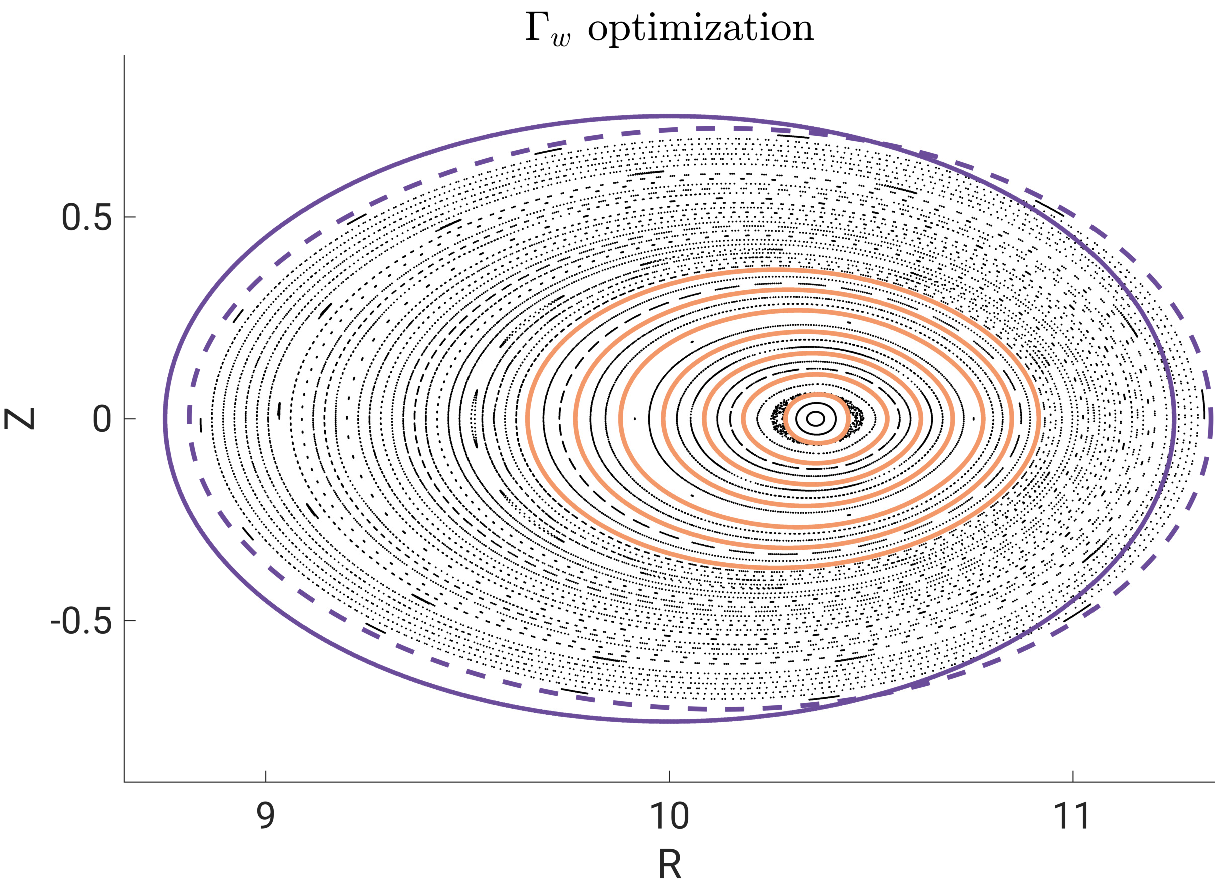
\includegraphics[width=.45\textwidth]{main/Figures_Optimization/BoundaryOptimization_Poincare.pdf}}
\hfill
\caption{Poincare section of the initial and optimized equilibria. Top left: Initial equilibrium (free-boundary and perfectly conducting wall cases). Red magnetic surfaces are SPEC's interfaces which support the pressure jumps. Purple interface is $\Gamma_{CB}=\Gamma_w$, outermost red interface is $\Gamma_{PB}$. Top right: free-boundary equilibrium, optimization of $\{V_{mn}\}$. In purple: $\Gamma_{CB}$ is the same as the initial $\Gamma_{CB}$. In yellow:  inner interfaces. Bottom left: optimization of $\{I^v_{\phi,l}\}_{l=\{1,\ldots,7\}}$. In purple: $\Gamma_w$ is the same as the initial equilibrium. In blue: inner interfaces. Bottom right: optimization of $\Gamma_w$. In purple (dashed): optimized $\Gamma_w$, in purple (full): initial $\Gamma_w$ and in orange: inner interfaces.}
\label{fig:poincare_plots}
\end{figure*}


\section{Perfectly conducting wall optimization}

 We now look at two different optimizations of the perfectly conducting wall equilibrium. In the first one, we only target the residues in the vacuum region, \textit{i.e.} residues with indices 1-3 of Table \ref{tab:residues}, and the parameter space is the profile of current flowing in the plasma volumes $\{I^v_{\phi,l}\}_{l=\{1,\ldots,7\}}$. When more residues listed in Table \ref{tab:residues} are included in the objective function, the optimizer is not able to lower the objective function sufficiently to observe an effect on the island width. This might be because not enough degrees of freedom were provided. Increasing the number of volumes $N_{vol}$ in \ac{SPEC}, consequently increasing the number of degrees of freedom $\{I^v_{\phi,l}\}_{l=\{1,\ldots,N_{vol}\}}$, is however not a guaranteed solution, since it adds additional topological constraints on the magnetic field and some island chains might remain undetected. The optimization of the injected current profile $\{I^v_{\phi,l}\}_{l=\{1,\ldots,7\}}$ could however be combined with other parameters, for example the coil optimization with degrees of freedom $\{V_{mn}\}$, to target more residues. Note that this optimization could also be achieved in the initial free-boundary equilibrium, but the perfectly conducting wall equilibrium was considered here for simplicity.
 
 In the second optimization, all residues listed in Table \ref{tab:residues} are included in the objective function and the geometry of the perfectly conducting wall $\Gamma_w$ is optimized. The selected degrees of freedom are the modes $R^w_{mn}$ and $Z^w_{mn}$ with $(m,n)=(1,1),\ (1,2),\ (2,1)$. Low order Fourier modes are chosen for their capacity to penetrate deeper in the plasma \citep{Helander2014}. In principle, higher order Fourier modes could be used, however the required deviation from the initial state might need to be large to minimize the objective function and thus the optimum state difficult to find for the optimizer. Note that the poloidal angle defined by the Fourier representation of the perfectly conducting wall $\Gamma_w$ is generally not a straight-field line angle. Which Fourier mode $R^w_{mn}$ and $Z^w_{mn}$ affects the targeted rationals is thus a non-trivial question --- in general, the residue associated to the $n/m$ rational might not be affected by the modes $\{R^w_{mn},Z^w_{mn}\}$!

Figure \ref{fig:poincare_plots} shows the result of the optimization of $\{I^v_{\phi,l}\}_{l=\{1,\ldots,7\}}$ (bottom left) and the optimization of $\Gamma_w$ (bottom right). Comparing both Poincare plots with the initial equilibrium (top left), we observe that the targeted residues have indeed been minimized - the islands are now much smaller, and are no longer visible in some cases.

The rotational transform profiles are plotted on Figure \ref{fig:iota_profile} and the total enclosed toroidal current on Figure \ref{fig:Iprofile}. Again, the rotational transforms are of the same order as for the unoptimized case. Regarding the optimized current profile, the total injected current is $\Delta I_\phi=-5.2$kA, less than $20\%$ of the initial total enclosed toroidal current. Interestingly, the optimizer found an equilibrium close to the initial state, and did not converge to the obvious global minimum, where a large toroidal current would be injected in the volumes to lift the rotational transform profile in order to push all the targeted rationals out of the plasma. Similarly, for the optimization of $\Gamma_w$, a trivial solution would be the axisymmetric solution, with $R^w_{mn}=Z^w_{mn}=0$ for $n\neq 0$. Again, since a local optimizer is being used, the optimum found is a local optimum close to the initial state, and not the global optimum.

\begin{figure*}
    \centering
    \hfill
    \subfloat[][]{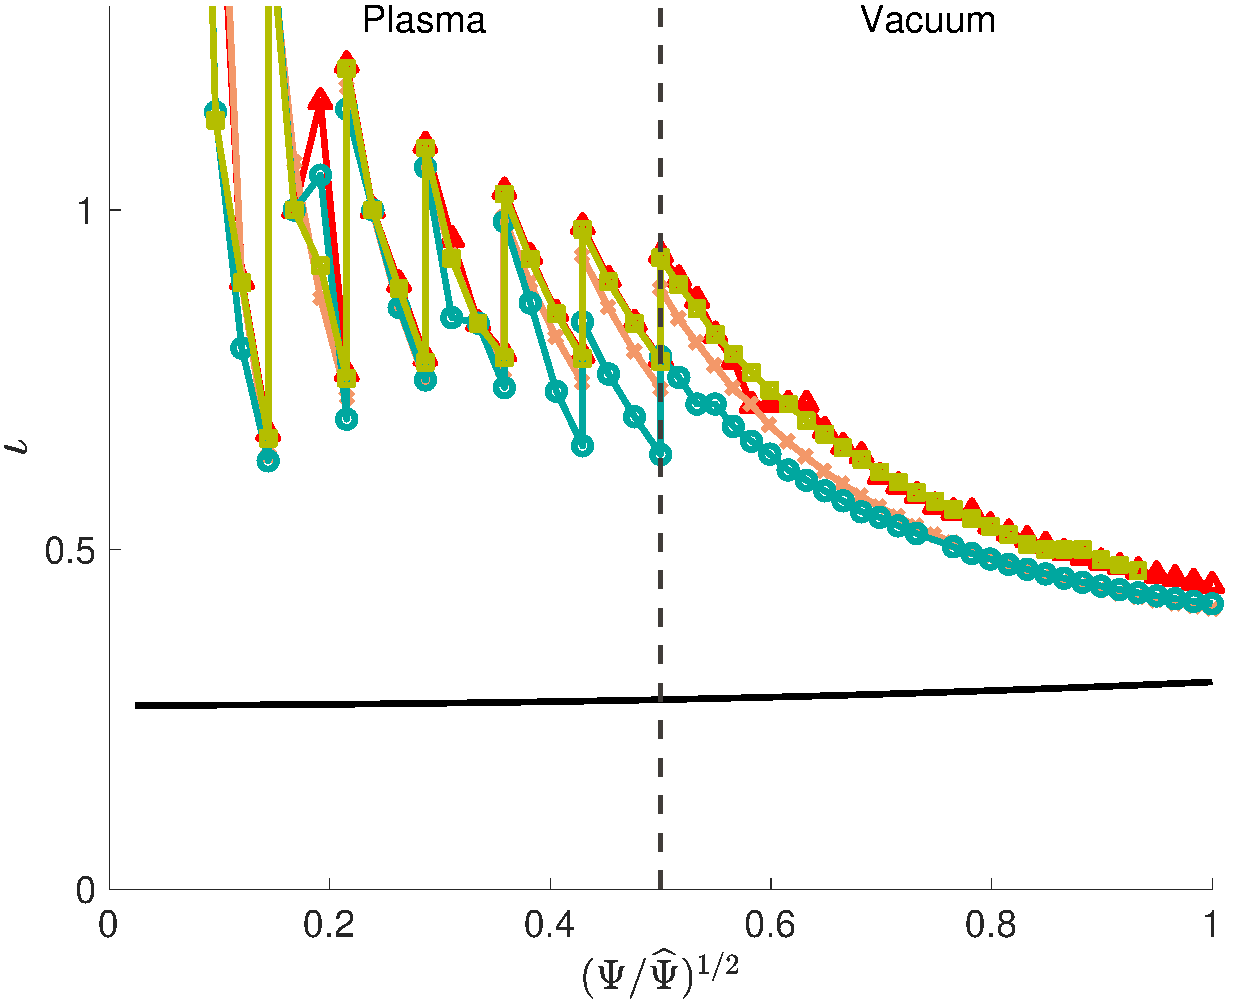
\includegraphics[width=.45\textwidth]{main/Figures_Optimization/IotaProfiles.pdf}}
    \hfill
    \subfloat[][]{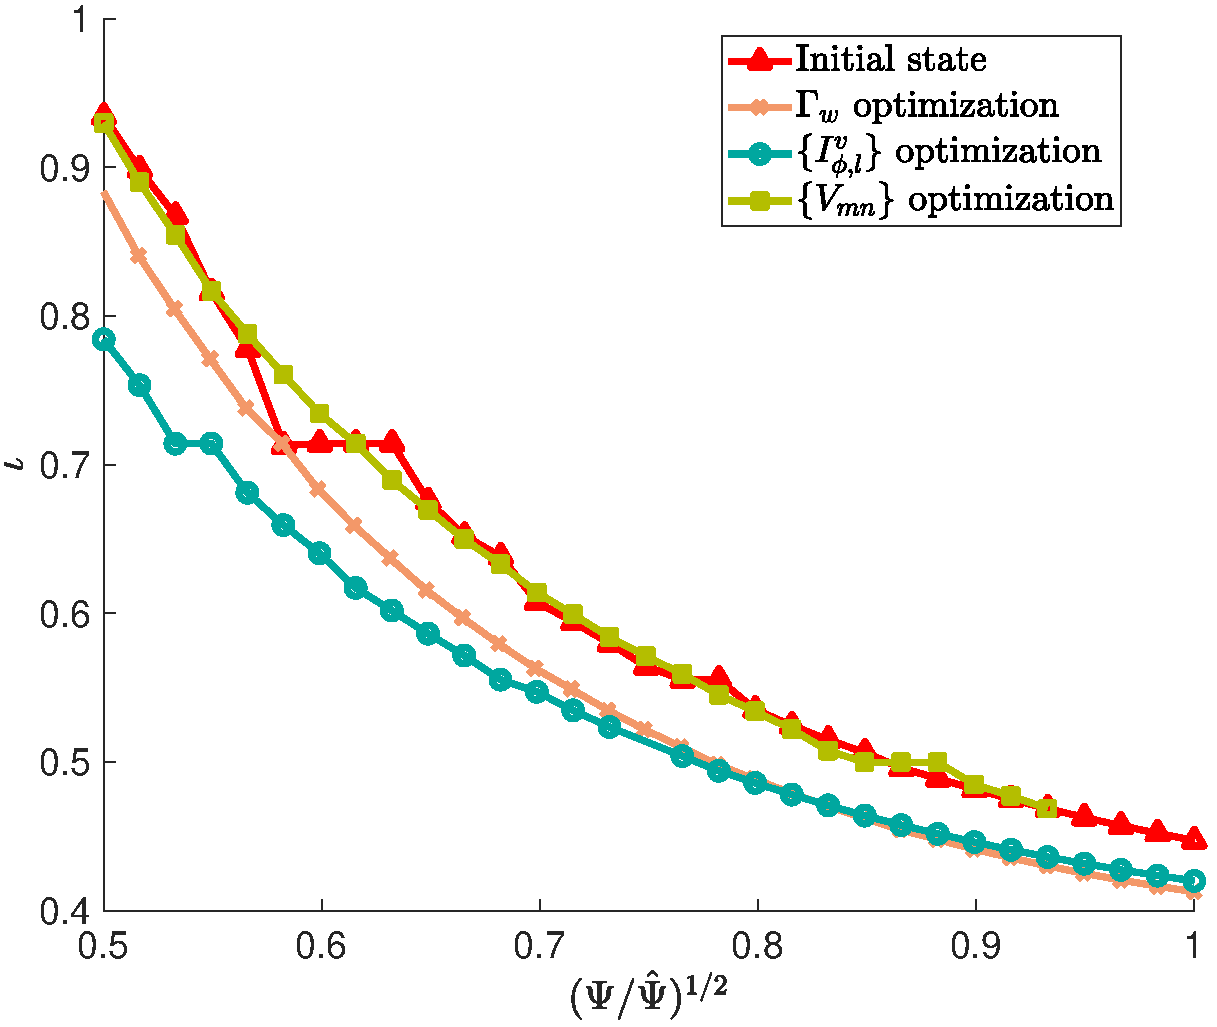
\includegraphics[width=.45\textwidth]{main/Figures_Optimization/IotaProfiles_Zoom.pdf}}
    \hfill
    \caption{Rotational transform as a function of the square-root of the normalized toroidal flux. Left: Full profile. Black, dashed line: position of the plasma-vacuum interface. Black, full line: vacuum profile. Right: zoom on vacuum region.}
    \label{fig:iota_profile}
\end{figure*}

\begin{figure}
    \centering
    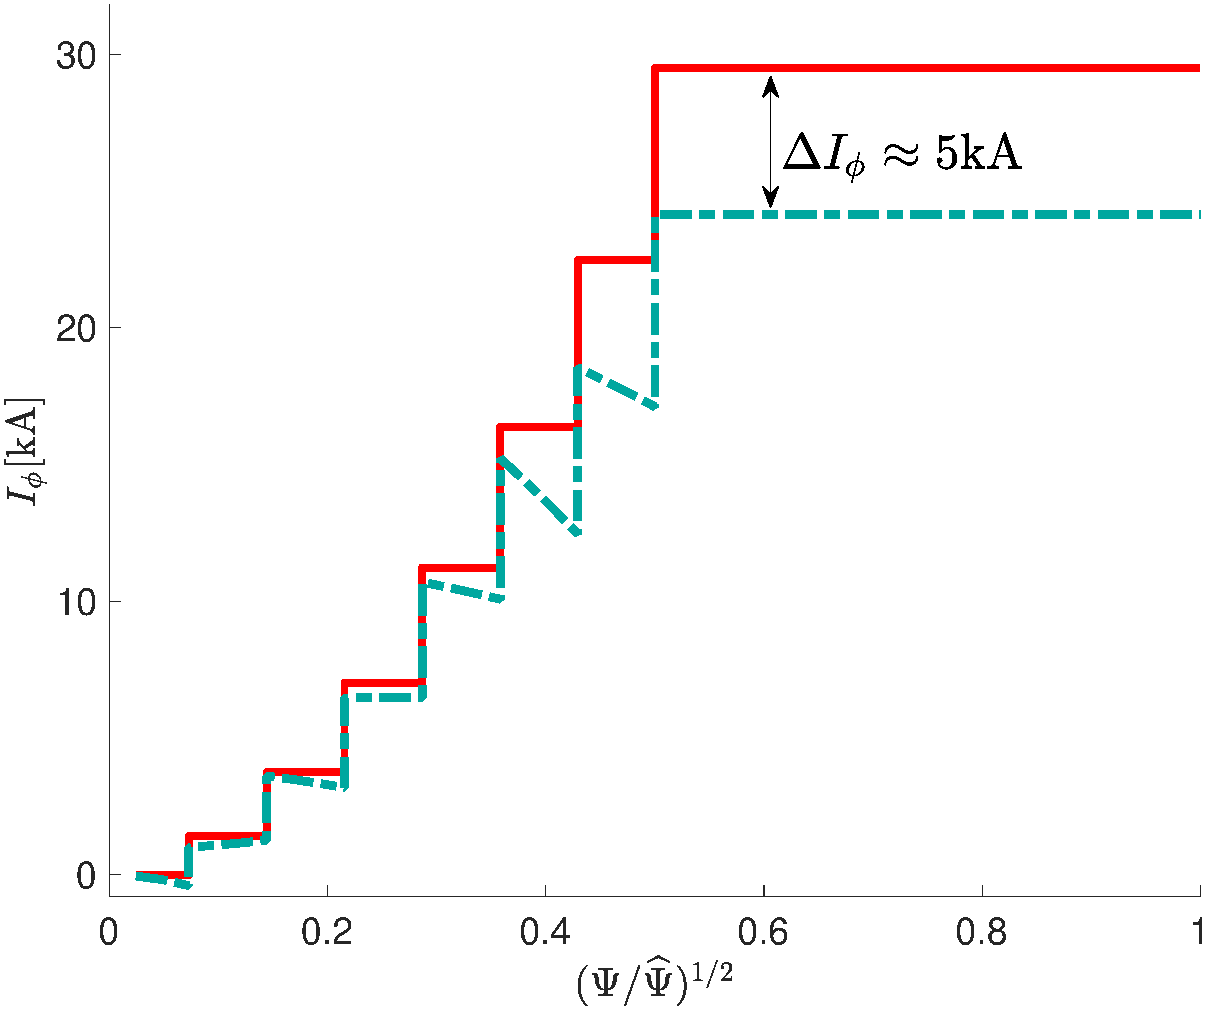
\includegraphics[width=.45\textwidth]{main/Figures_Optimization/CurrentProfiles.pdf}
    \caption{Total enclosed toroidal current as a function of the square-root of the normalized toroidal flux. In red: initial equilibrium and in blue: $\{I^v_{\phi,l}\}_{l=\{1,\ldots,7\}}$ optimized equilibrium. Other optimized equilibria have the same toroidal current profile as the initial equilibrium, and are thus not plotted. }
    \label{fig:Iprofile}
\end{figure}





\section{Convergence and computation time}

The normalized value of the objective function as a function of the number of iterations is plotted for each optimization in Figure \ref{fig:objective_function}. The optimization of $\Gamma_w$ (orange crosses) can not be compared with the other two, since it uses a different objective function. We see that the optimization of $\{I^v_{\phi,l}\}_{l=\{1,\ldots,7\}}$ (blue circles) saturates at a larger value than the optimization of $\{V_{mn}\}$ (green squares), despite optimizing the same objective function (the same residues were selected). Intuitively, this can be understood by noticing that the number Fourier harmonics of the magnetic field that are affected by the plasma current is smaller than those that can be affected by the $\{V_{mn}\}$. In that sense, the space of possible perturbations of the magnetic field for influencing the islands is more constrained in the $\{I^v_{\phi,l}\}_{l=\{1,\ldots,7\}}$ optimization.

The optimization was run in parallel on $2n+1$ cores of Intel Broadwell processors at 2.6GHz, where $n$ is the number of degrees of freedom of the optimization. Each core computed a different SPEC equilibrium when evaluating the finite difference estimate of the objective function gradient. The $\{V_{mn}\}$ optimization required $165$ equilibrium calculations, the $\{I^v_{\phi,l}\}_{l=\{1,\ldots,7\}}$ optimization  $187$ and the $\Gamma_w$ optimization $309$. The total CPU time for execution was respectively $\sim41$ days, $\sim10$ days and $\sim21$ days for a total wall-clock time of respectively $\sim 65$h, $\sim 17$h and $\sim 39$h. As expected, the optimizations of the perfectly conducting wall equilibrium were faster, as fixed-boundary calculations are faster than free-boundary ones. 

Note that the presented optimizations did not take advantage of the full parallelization of \ac{SPEC} --- only a single core computed each \ac{SPEC} equilibrium, while SIMSOPT allows the user to use $M\le N_{vol}$ \acp{CPU} on $N\le 2n+1$ \ac{SPEC} instances, which would speedup the computation greatly. Nevertheless, our optimizations show that the total time required to perform a SPEC optimization is small enough to be considered in more advanced stellarator optimizations.

\begin{figure}
    \centering
    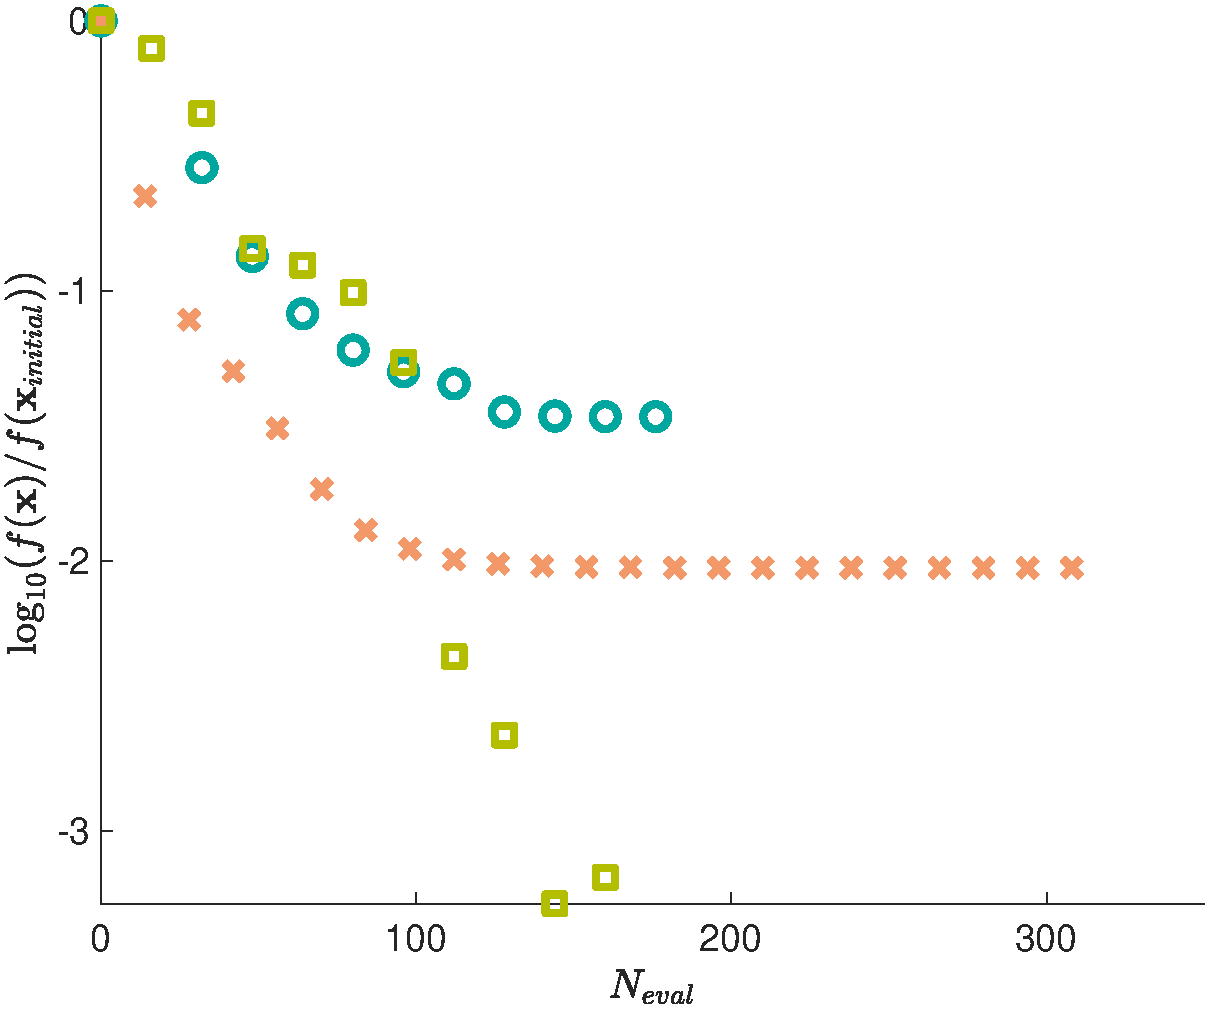
\includegraphics[width=.45\textwidth]{main/Figures_Optimization/ObjectiveFunction.pdf}
    \caption{Logarithmic plot of the normalized objective function as a function of the number of \ac{SPEC} calculations. Orange crosses: optimization of $\Gamma_w$. Blue circles: optimization of $\{I^v_{\phi,l}\}_{l=\{1,\ldots,7\}}$. Green squares: optimization of $\{V_{mn}\}$.}
    \label{fig:objective_function}
\end{figure}




\section{Optimization of the equilibrium $\beta$-limit}

We propose here to optimize a sequence of equilibria at different values of $\beta$ to increase the configuration equilibrium $\beta$-limit. 



\section{Conclusion}

In this paper, we showed the first fixed- and free-boundary, multi-volume, finite $\beta$ \ac{SPEC} equilibrium optimizations of a classical stellarator using the SIMSOPT framework. The objective function was constructed from the Greene's residues of selected rational surfaces. Different parameter spaces were considered: either the boundary of a perfectly conducting wall surrounding the plasma, or the enclosed toroidal current profile, or the vacuum field produced by the coils were optimized. 

In all three optimizations, it was possible to reduce the objective function significantly, which in turn translated to a reduction of the targeted magnetic island width. In the case of the current profile optimization, the volume occupied by magnetic islands and chaotic field lines was considerably reduced in the vacuum region surrounding the plasma. While not important for plasma confinement, the control of the magnetic field topology in the vacuum region is of paramount importance for divertor design and operation. In the case of the perfectly conducting wall optimization, the volume occupied by magnetic surfaces was increased both in the vacuum region and in the plasma volume. Finally, in the case of the optimization of the vacuum field produced by the coils, the islands present in the initial unoptimized equilibrium were reduced in size, but additional rationals and island chains emerged, since their associated residues were not included in the objective function. 

Different measures of the magnetic field integrability are currently being considered to overcome the shortcomings of Greene's residues. Indeed, as observed in the coil optimization, Greene's residue is a local measure, which requires input from the user --- any rational surface emerging during the optimization remains undetected. Ideally, a global measure is thus required. The volume occupied by chaotic field lines, measured from the fractal dimension of their Poincare map \cite{Loizu2017} could be a possible solution. 

In the work by \citet{Landreman2021a}, it has been shown that \ac{SPEC} could be coupled to VMEC in order to achieve an optimization in a vacuum, where both quasi-symmetry and nested flux surfaces could be obtained. The obvious next step is then to perform a combined \ac{SPEC}-VMEC finite-$\beta$ optimization for good magnetic surfaces as well as other metrics, such as quasi-symmetry. This will require to deviate significantly from a classical stellarator geometry, as opposed to what has been presented in this paper, and the computational cost of the optimization will be greater due to the increased complexity of the problem. While this task does not require extensive development of the optimization tool SIMSOPT, a number of convergence issues in SPEC arising in strongly shaped geometries have to be solved. Alternative Fourier representations of the volumes interfaces \citep{Henneberg2021} are currently being implemented to attempt to solve this issue. This will be the topic of future investigations.

%
% ****** End of file aipsamp.tex ******

\end{document}